\chapter{Measurement of \kcharged production in pp collisions}
\label{cap:5}
\vspace*{2cm}
\kstarch~is a resonance particle with a small lifetime ($\sim$ 4~\fmc), comparable to that of the fireball which is produced during the heavy ion collision. Due to its short lifetime, it can be used to study the re-scattering and regeneration effects. \kstarch~can provide the information regarding strangeness enhancement as it contains a strange quark. Measurements of \kstarch~in pp collisions can be used as a baseline to study the \PbPb~collisions at the LHC energy and to provide a reference for tuning event generators.  
This note describes the measurement of \kstarch~mesons (in the following \simplekstarch) produced at mid-rapidity (\modrap~$\leq$~0.5) in minimum-bias pp collisions at \sqrtS~=~13~TeV. In this analysis, \simplekstarch~has been reconstructred by its hadronic decay chanel \kstarch $\rightarrow$  \ppm + \kshort. The yield of \simplekstarch~is extracted from \pion\kshort~invariant-mass distributions as a function of transverse momentum. 
The \pT~spectrum is integrated to obtain a measurement of the total \dndy, and the mean transverse momentum \meanpT~is extracted from the spectrum. 


\section{\kzero reconstruction in pp collisions}
\label{par:5.1}
The \kcharged~ production in pp collisions at \sqrtS~= 13 TeV has been done with data collected in 2015 by ALICE detector. The analysis strategy is based on the invariant mass study of reconstructed pairs whose origin could be the decay of \kzero~ mesons into charged particles. The daughter particles are identified as oppositely charged pions and kaons among the tracks reconstructed in the central barrel. Track selection and particle identification is described further in this chapter. To extract the yields of \kzero~ mesons in each \pT~ bin, the invariant-mass distribution of unlike-charge pairs from the same event is computed. The combinatorial background is estimated by event-mixing technique and subtracted from the unlike-charge distribution. In event-mixing technique, the combinatorial background is constructed through the invariant mass of pions and kaons of different events having similar z-vertex, and multiplicity. The mixed event is normalised by the same event distribution in the region of invariant mass of 1.1 to 1.3 \GeVcSq. The signal is obtained by subtracting the mixed event combinatorial background from the same event kaon - pion invariant mass distribution. (see \mbox{Figure \ref{Fig:chap5-5.1}})

\begin{figure}[ht]
\centering
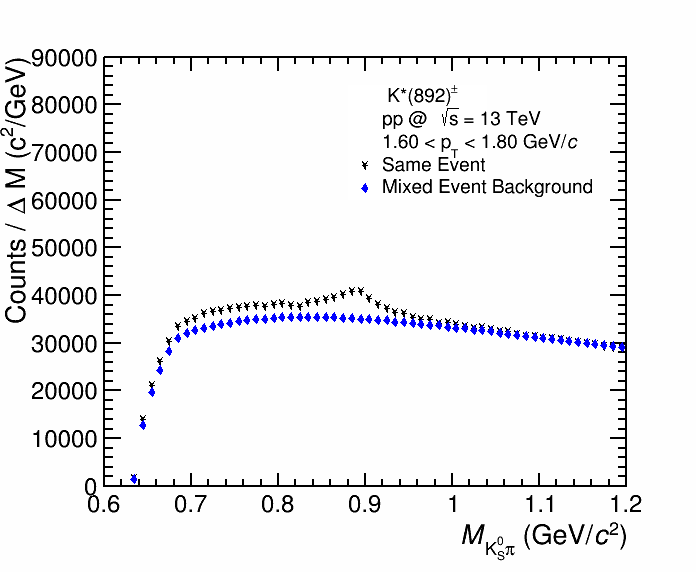
\includegraphics[width= 0.425\textwidth]{Images/Chapter5/inv_mass/invmass6.png}
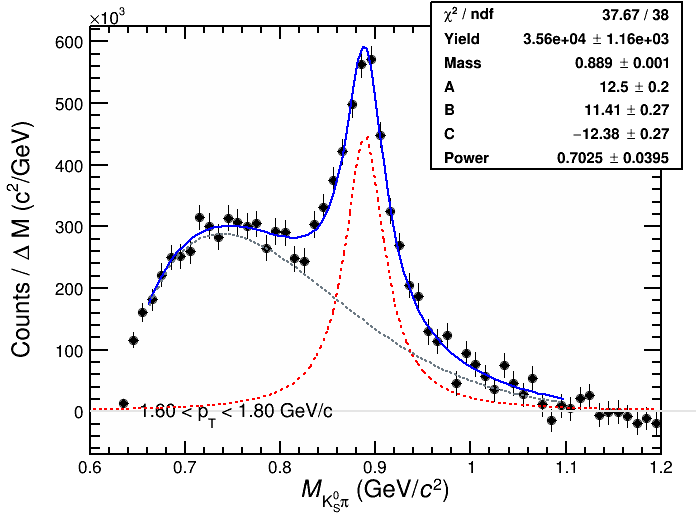
\includegraphics[width= 0.45\textwidth]{Images/Chapter5/Signal/signal6.png}
\caption{(Left panel) The \kshort\ppm invariant mass distribution in \modrap~$<$~0.5 for the bin 
1.6~$<$~\pT~$<$~1.8~\gmom~in pp collisions at \sqrtS~=~13~TeV. The background shape estimated using pairs from different events (event-mixing technique) is shown as open green circles. (Right panel) The \kshort\ppm~invariant mass distribution for the bin 1.6~$<$~\pT~$<$~1.8~\gmom~after background subtraction. The solid red curve is the results of the fit by eq.~\ref{eqn4}, the dashed blue (green) curve describes the residual background (Breit-Wigner distribution).}
\label{Fig:chap5-5.1} 
\end{figure}

\section{Data sample and event selection}
\label{par:5.2}

The data used for this analysis was taken during June 2015 pp run (LHC15f, pass 2 reconstruction \footnote{A few reconstruction processes are needed to obtain data usable for physics analysis. Usually the first two reconstruction passes (pass $0$ and pass $1$) are needed for quality assurance check and calibration of the main detectors. The pass $2$ is the first usable reconstruction for analysis purpose. Further passes are needed to implement signals from detectors requiring special calibrations.}). The full sample consists of 104 runs totalling to about $527 \times 10^{6}$ events. Out of these, only 48 runs have been used, which are marked by the collaboration as 'good runs' i.e. they are characterized by good performance of the detectors and good running conditions (e.g. low level of beam induced background). In particular, all these \virgolette{good runs} have both the TPC and all the ITS sub-detectors turned on.


The purpose of the event selection is to select hadronic interactions with the highest possible efficiency, while rejecting the machine-induced and physical backgrounds. The ALICE on-line minimum bias (MB) trigger for this pp run was configured to require the following two conditions: 

\begin{description}
\item[(i)] a signal above the threshold in V0A,
\item[(ii)] a signal above the threshold in V0C.
\end{description}


The threshold in the VZERO detector corresponds approximately to the energy deposition of a minimum ionizing particle. 


For this analysis, a sample of $45 \times 10^{6}$ minimum bias pp events has been processed where ITS, TPC and TOF performance was optimal. Out of this, around 16 million events satisfy the following selection criteria and have been actually used for the analysis:

\begin{itemize}
\item Is InComplete DAQ check.
\item Pileup Rejection using AliAnalysisUtils::IsPileUpEvent().
\item SPD Clusters vs. Tracklets Check using AliAnalysisUtils::IsSPDClusterVsTrackletBG() with default parameters.
\item Event has a track or SPD primary vertex identified.
\item SPD vertex-z resolution $< 0.25$ cm.
\item SPD vertex dispersion $< 0.04$ cm.
\item z-position difference between track and SPD vertex $< 0.5$ cm.
\item vertex-z position : $|v_{z}| < 10$ cm.
\end{itemize}



\begin{figure}[h!]
\centering
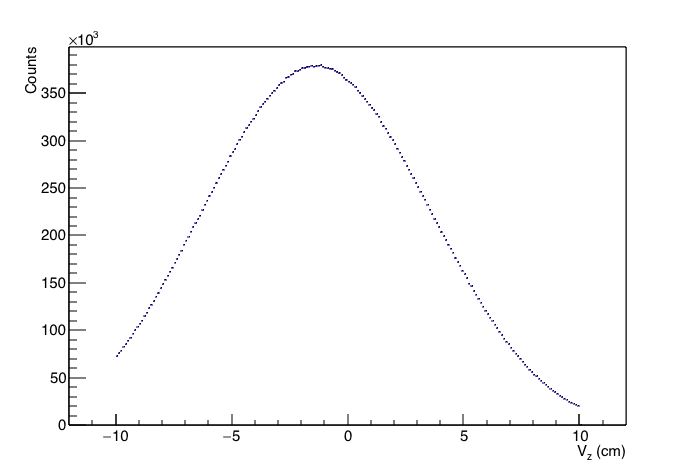
\includegraphics[width=0.7\textwidth]{Images/Chapter5/prim_vtx.png}
\caption{Vertex z coordinate distribution of the accepted events.} 
\label{Fig:chap5-5.2}
\end{figure} 


The distribution of vertex z position of the accepted events is reported in \mbox{Figure \ref{Fig:chap5-5.2}}. Events with $|V_z| < $ 10 cm have been used to ensure a uniform acceptance in the central pseudorapidity region, $|h| < $0.8, where the analysis is performed.

\section{\ensuremath{\pi^{\pm}}  and $\mathrm {K^0_S}$ selection}
\label{par:5.3}
The \kstarch~ mesons were identified by reconstructing their decay in a charged pion (\ppm) and a \kshort. Once identified a rapidity cut (\modrap~$<$~0.5) has been applied to the pairs \ppm\VZERO.

\subsection{Primary pion selection}
\label{par:5.3a} 
Primary charged tracks were selected by applying the following cuts:
	
\begin{itemize}
\item  \pT $>$ 0.15 \gmom 
\item -0.8 $< \eta <$ 0.8
\item Reject kink daughters
\item Minimum number of rows crossed in TPC is 70
\item Ratio of number of crossed rows to number of findable clusters in TPC $>$~0.8
\item Require TPC refit
\item Require ITS refit
\item TPC $\chi^{2}$ per clusters $<$~4.0
\item ITS $\chi^{2}$ per clusters $<$~36.0
\item $\chi^{2}$ per clusters in TPC-Constrained global fit $<$~36.0
\item Minimum number of clusters in SPD: 1 (AliESDtrackCuts::SetClusterRequirementITS(kSPD, kAny))
\item AliESDtrackCuts::SetDCAToVertex2D(kFALSE)
\item AliESDtrackCuts::SetRequireSigmaToVertex(kFALSE) 
\item $\left | \mathrm{DCA}_{\mathrm{z}} \right | <$~2~cm
\item $\mathrm{DCA}_{\mathrm{r}}<$ 0.0105+0.0350~\pT$^{-1.1}$ (a 7$\sigma$~\pT~dependent cut)
\end{itemize}

These cuts, but the first two, are included in the function 
 
\textbf{AliESDtrackCuts:GetStandardITSTPCTrackCuts2011(kTRUE, 1)} which implements the standard ITS/TPC track cuts from 2011.

The primary pions were identified through their energy loss \dedx~in the Time Projection Chamber (TPC). For this analysis due to problem with TPC PID  wider TPC cuts were used at low momentum. The following  $p$-dependent PID selection cuts were applied: 


\begin{itemize}
\item $\left | \mathrm{N\sigma}_{\mathrm{TPC}} \right | < $ 6 for $p$ $<$ 0.3 \gmom
\item $\left | \mathrm{N\sigma}_{\mathrm{TPC}} \right | < $ 4 for 0.3 $\leq p \leq$ 0.4~\gmom
\item $\left | \mathrm{N\sigma}_{\mathrm{TPC}} \right | < $ 3 for $p >$ 0.4~\gmom
\end{itemize}
 
In \mbox{Figure \ref{Fig:chap5-5.3}}) $\mathrm{N\sigma}_{\mathrm{TPC}}$ versus momentum $p$ for pions without any PID cut (left panel) and after that $p$-dependent PID cut is applied (right panel) are shown.

\begin{figure*}[h]
\centering
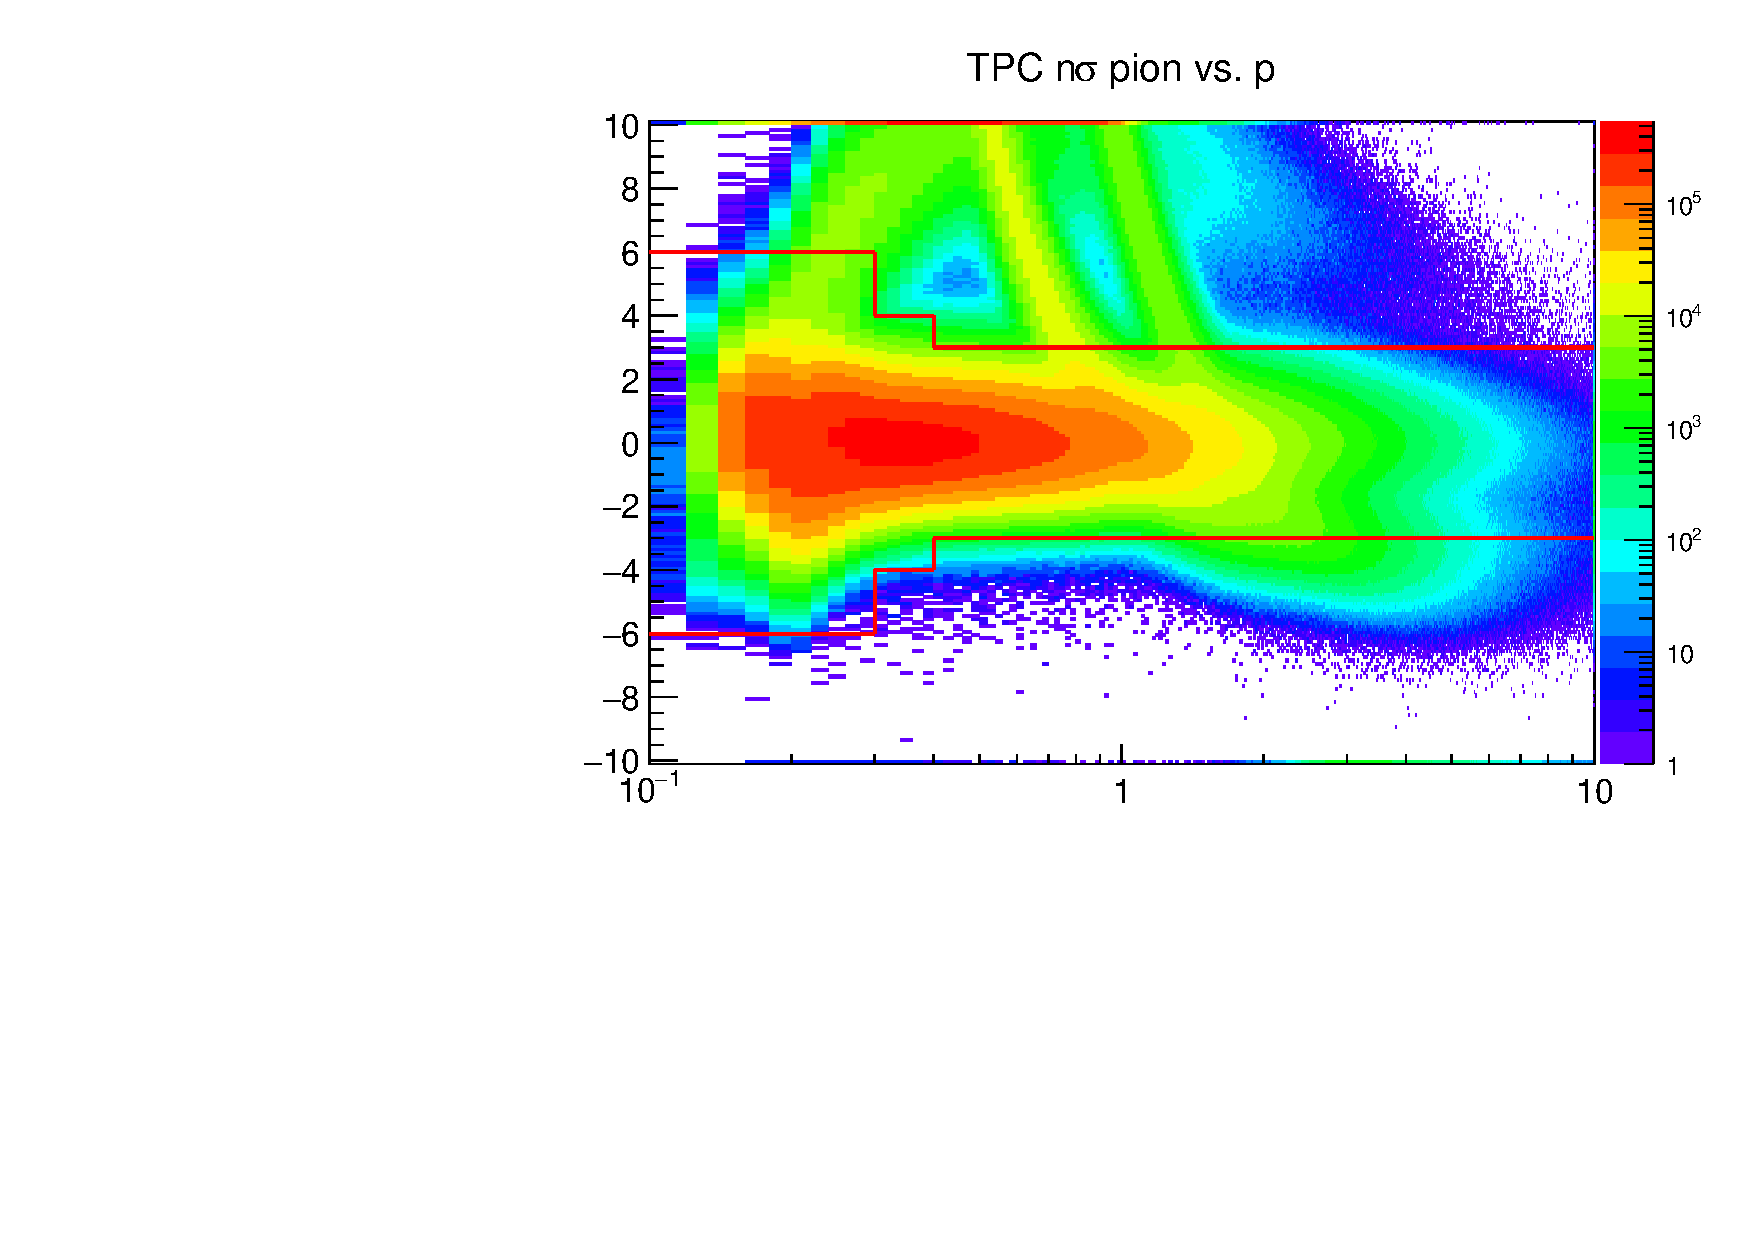
\includegraphics[width= 0.42\textwidth]{Images/Chapter5/pion_TPC.pdf}
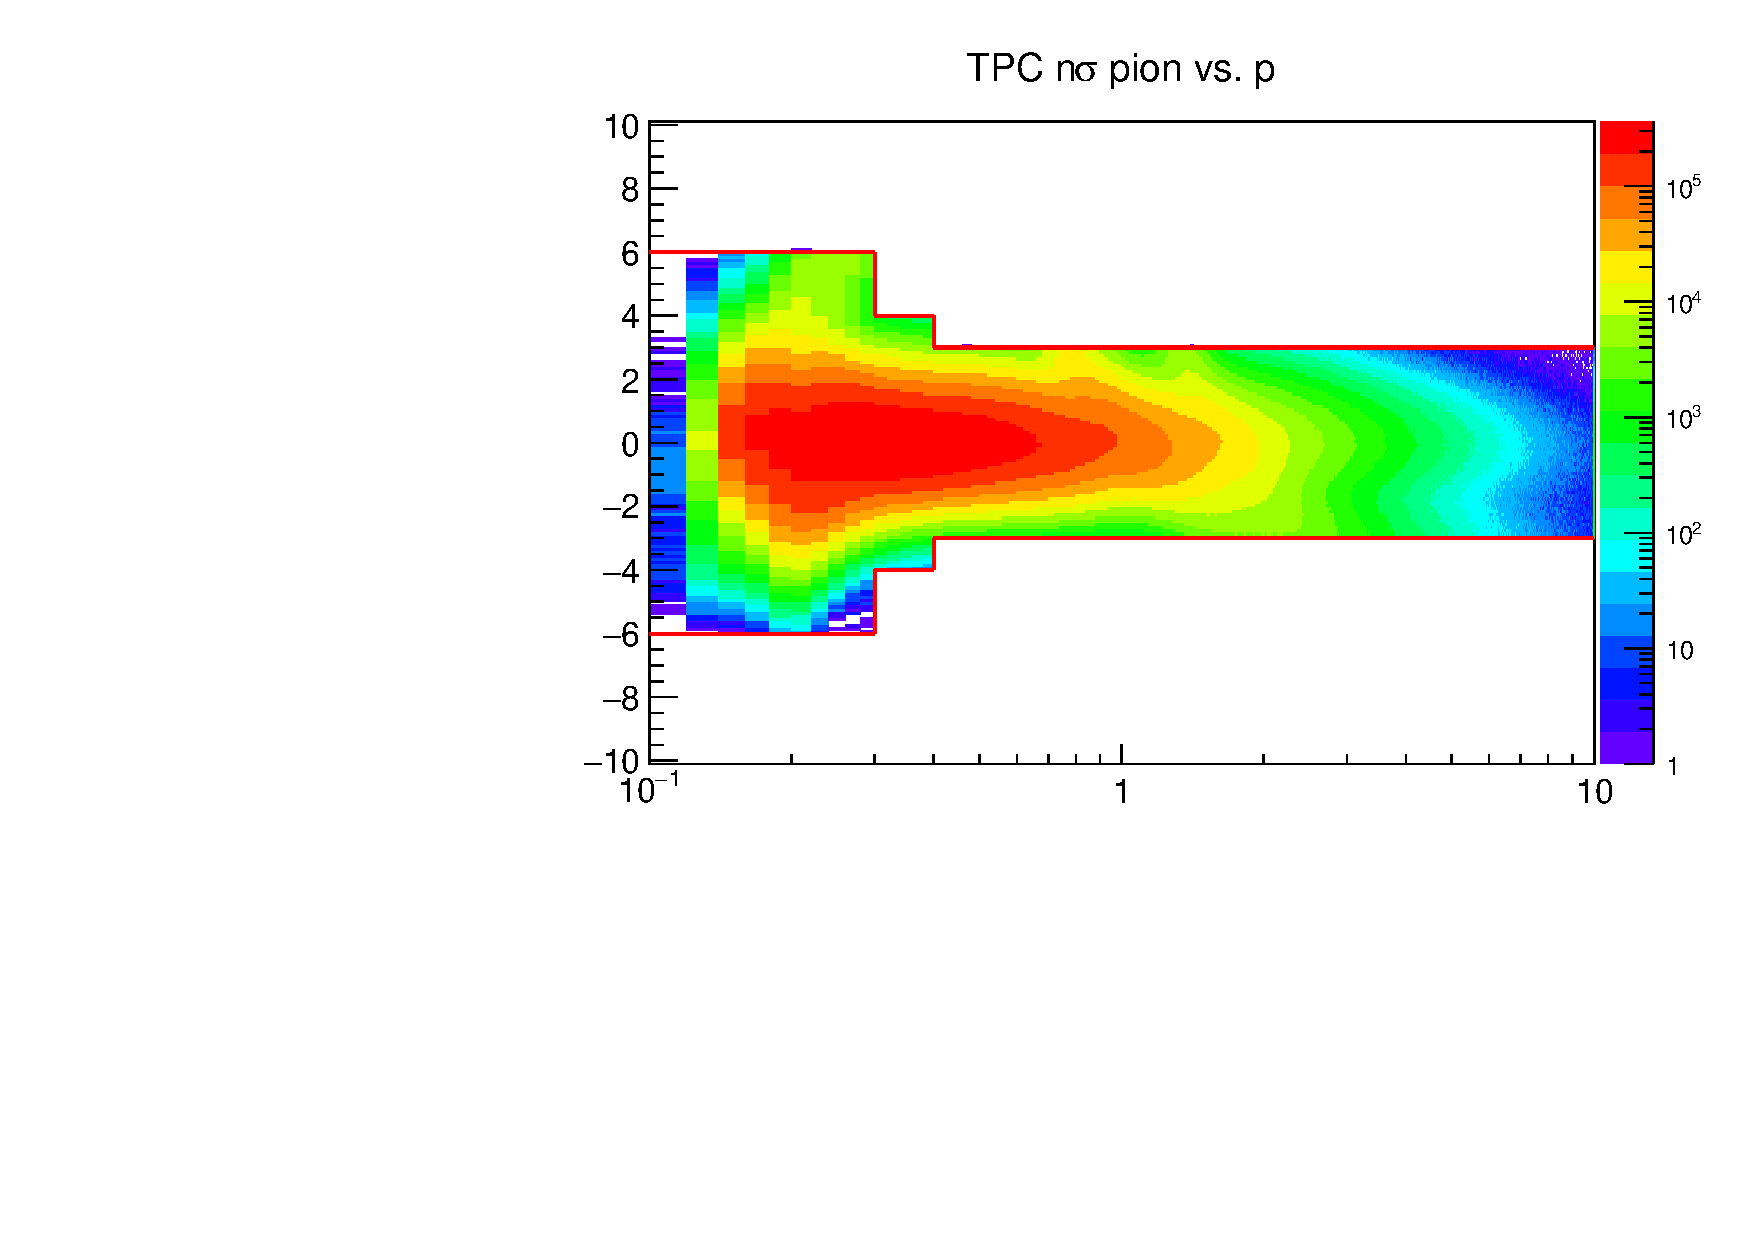
\includegraphics[width= 0.42\textwidth]{Images/Chapter5/pion_TPC_cut.pdf}
\caption{$\mathrm{N\sigma}_{\mathrm{TPC}}$ versus momentum $p$ for pions without any PID cut (left panel) and after $p$-dependent PID cut is applied (right panel). The dotted lines indicate the TPC PID cuts as a function of momentum.}
\label{Fig:chap5-5.3} 
\end{figure*}
 
\subsection{\VZERO~selection}
\label{par:5.3b} 
The \VZERO~\kshort~is identified by its decay \kshort $\rightarrow$  \pip + \pim.

The following selection criteria were applied to select the secondary pions. 
 
\textbf{Daughter track selection criteria}
\begin{itemize}
\item $-0.8<\eta <0.8$
\item Require TPC refit
\item Reject Kink Daughters
\item Minimum number of rows crossed in TPC $>$~70
\item Ratio of number of crossed rows to number of findable clusters in TPC $>$~0.8
\item TPC $\chi^{2}$/clusters $<$~4.0
\item DCA of tracks to PV $>$ 0.0105+0.0350~\pT$^{-1.1}$~cm  (a \pT~dependent cut to be complementary to primary tracks)
\end{itemize}

Furthermore secondary pions were identified through their energy loss \dedx~in the Time Projection Chamber (TPC), by a wide PID cut $\left | \mathrm{N\sigma}_{\mathrm{TPC}} \right | < $ 5.

The pairs of \pip\pim~which fulfill the following \textbf{\VZERO~selection criteria} were taken as \kshort~candidates

\begin{itemize}
\item Only Offline \VZERO
\item Rapidity \modrap $<$~2.0
\item Fiducial Volume (\VZERO~2D decay radius) $>$~0.5~cm
\item \VZERO~cosine of pointing angle $>$~0.97
\item DCA \VZERO~to Primary Vertex $<$0.3~cm
\item DCA \VZERO~daughters $<$ 1.0~$\sigma$
\item \VZERO~Mass Tolerance $<$~0.03~\gmass 
\item Proper Lifetime ($mL/p$) $<$~20~cm 
\end{itemize}

The previous cuts are the same used for the identification of \kshort~in pp collisions at \sqrtS~=~13~TeV. Only difference is for the \VZERO~mass cut. A \VZERO~mass tolerance cut was added to well select \kshort~particles. On the contrary, the competing \VZERO~rejection was not used since a slightly decrease of the signal without any increasing of its significance was observed. In case this rejection is used only pairs that have an invariant mass incompatible with the hypothesis to be originated from a \rmLambda~or {\rmAlambda~decay ($\left | \mathrm{M}_{\mathrm{\rmLambda}} - 1115.683 \right | > $~4~\mmass~or  
$\left | \mathrm{M}_{\mathrm{\rmAlambda}} - 1115.683 \right | > $~4~\mmass) would be taken.  Furthermore considering that we are interested only to "primary" \VZERO~a cut of 0.3~cm was applied on the DCA of the \VZERO~to the primary vertex.     




